\documentclass[parskip=full]{scrartcl}
\usepackage{pdfpages}
\usepackage[utf8]{inputenc}
\usepackage[T1]{fontenc}
\usepackage[german]{babel}
\usepackage{hyperref}
\hypersetup{
	pdftitle={Pflichtenheft},
	bookmarks=true,
}
\usepackage{csquotes}

\usepackage{fancyhdr}%<-------------to control headers and footers
\usepackage[a4paper,margin=1in,footskip=.25in]{geometry}
\fancyhf{}
\fancyfoot[C]{\thepage} %<----to get page number below text
\pagestyle{fancy} %<-------the page style itself

\usepackage{xcolor}
\usepackage{framed}
\definecolor{shadecolor}{RGB}{220,220,220}
\usepackage{float}


\title{Android GO! App - Pflichtenheft}
\author{Gruppe 3}
\date{11.06.17}

% define custom lists
\usepackage{enumitem}
\usepackage{lipsum}

% add glossary
\usepackage{glossaries}
\makeglossaries
\newglossaryentry{System}
{
	name={System},
	description={Die Kombination aus Mobile App und Server},
}
\newglossaryentry{GO-Lifecycle}
{
	name={GO-Lifecycle},
	description={Der gesamte Zeitraum von der Erstellung bis zur Beendigung des GOs},
}

\newglossaryentry{GO} %TODO anderen Namen finden
{
	name={GO},
	description={Ein Event in einer Gruppe, dem Mitglieder beitreten können, um ihren Standort mit anderen GO-Teilnehmern zu teilen},
	plural={GOs},
}
\newglossaryentry{Benutzer}
{
	name={Benutzer},
	description={Eine Person, die die App installiert und sich mit einem Benutzeraccount registriert hat bzw. plant dies zu tun},
}
\newglossaryentry{Benutzername}
{
	name={Benutzername},
	description={Ein im System nicht-eindeutiger Name, den der Benutzer jederzeit ändern kann},
}
\newglossaryentry{Hauptansicht}
{
	name={Hauptansicht},
	description={Ansicht, die geöffnet wird, sobald sich ein Benutzer angemeldet hat. Dies entspricht der Ansicht in Abbildung \ref{hauptansicht}},
}
\newglossaryentry{App}
{
	name={App},
	description={mobile Applikation, die auf dem Smartphone/Tablet des Benutzers installiert ist. Der Benutzer interagiert ausschließlich mit der Applikation und nicht mit dem Webserver direkt},
}
\newglossaryentry{losgehen}
{
	name={losgehen},
	description={Die Änderung des Teilnahmestatus eines GOs von 'Bestätigt' auf 'Unterwegs'},
}
\newglossaryentry{Google-Account}
{
	name={Google-Account},
	description={Ein Benutzeraccount bei dem Internetdienstleister Google, die Benutzerkennung besteht aus einer E-Mailadresse mit der Domain '@gmail.com' und einem Passwort}
}
\newglossaryentry{Clustering}
{
	name={Clustering},
	description={Clustering bezeichnet den Vorgang, nahe beieinander gelegene Datenpunkte (im Kontext der App sind dies die Standorte der GO-Teilnehmer) zu einer Gruppe (sprich einem Cluster) zusammenzufassen}
}
\newglossaryentry{Android-Benachrichtigung}
{
	name={Android-Benachrichtigung},
	description={Benachrichtigungen, die dem Benutzer auf dem Smartphone-Bildschirm angezeigt werden, soblad etwas Neues in der App passiert ist. Dies erfordert nicht das Öffnen der App},
	plural={Android-Benachrichtigungen}
}
\newglossaryentry{GO-Teilnehmer}
{
	name={GO-Teilnehmer},
	description={Ein Mitglied der zu dem GO gehörigen Gruppe, dessen Teilnahmestatus 'Bestätigt' oder 'Unterwegs' lautet},
}


\def\threedigits#1{%
  \ifnum#1<100 0\fi
  \ifnum#1<10 0\fi
  \number#1}

\begin{document}

\begin{titlepage}
	\begin{center}
	%TODO evtl App-Logo ergänzen
	%\includegraphics[width=0.15\textwidth]{example-image-1x1}\par\vspace{1cm}
	{\scshape\LARGE \bfseries Pflichtenheft \par}
	\vspace{1cm}
	{\scshape\Large Praktikum der Softwareentwicklung \\ Sommersemester 2017\par}
	\vspace{1.5cm}
	{\huge\bfseries Android GO! App\par}
	\vspace{2cm}
	{\Large\itshape - Gruppe 3 -\par}
	\vfill
	{\bfseries erstellt von:\par}
	Arsenii Dunaev \\
	Florian Kröger \\
	Tina Maria Strößner \\
	Volodymyr Shpylka \\	
	\vfill
	% Bottom of the page
	{\large 11.06.17 \par}	
	\end{center}
\end{titlepage}

\tableofcontents

%TODO Gliederung ggfs nochmal überarbeiten
\newpage
\section{Zielbestimmung}
Die \gls{App} dient der Erleichterung und Strukturierung von Gruppentreffen. 
 Bei täglichen Vereinbarungen ist die Kommunikation im Text-Format via WhatsApp und ähnlichen Apps unübersichtlich und unintuitiv. 
Dieses Problem wird durch die GO-App gelöst, indem wir Struktur in den Vereinbarungsprozess reinbringen.  
\subsection{Musskriterien}

\begin{itemize}[itemsep=0pt]
	\item Der Benutzer  
	\begin{itemize}
		\item Unterscheidung zwischen Administrator der Gruppe und ordentlichen Teilnehmer der Gruppe.
		\item Unterscheidung zwischen GO-Verantwortlichen und ordentlichen Teilnehmer der Gruppe.
	 	\item Der App-Benutzer kann sich in der App registrieren und damit einen Benutzeraccount erstellen.
	 	\item Der Benutzer kann sich mithilfe von Google-Account im \gls{System} anmelden und vom System abmelden.
	 	\item Der Benutzer kann seinen Benutzeraccount löschen.
	 	\item Der Benutzer kann die 'About'-Seite einsehen.
	 	\item Der Benutzer kann Lizenzinformationen einsehen.
	\end{itemize} 
	
	\item Die Gruppen
	\begin{itemize}
	 		%\item Jeder kann eine Gruppe erstellen und Nutzer in die Gruppe einladen
	 		%\item Jeder Teilnehmer der Gruppe kann ein Event in der Gruppe erstellen
	 		%\item Jeder Teilnehmer der Gruppe kann sich zum Event in der Gruppe anschließen
	 		%Das oben kommentiert sind eher schon Funktionalen Anforderungen
	 	\item Der Benutzer kann eine Anfrage auf Gruppenmitgliedschaft beantworten.
	 	\item Der Benutzer kann eine Gruppe erstellen.
	 \end{itemize}
	 Die folgenden Kriterien funktionieren lediglich in den Gruppen, in denen der Benutzer Mitglied ist.
	 \begin{itemize}
	 	\item Der Benutzer kann alle seinen Gruppen einsehen.
	 	\item Der Benutzer kann die Systeminformationen zu den Gruppen einsehen.
	 	\item Der Benutzer kann aus der Gruppe austreten.
	\end{itemize}
	
	\item Der Administrator der Gruppe\\
	Die folgenden Kriterien funktionieren lediglich in den Gruppen, in denen der Benutzer Mitglied und gleichzeitig Administrator ist.
	\begin{itemize}
		\item Der Administrator kann Gruppendaten ändern.
		\item Der Administrator kann der Gruppe neue Mitglieder hinzufügen.
		\item Der Administrator kann Mitglieder der Gruppe entfernen.
		\item Der Administrator kann die Gruppe löschen.  
	\end{itemize}
	
	\item Die \glspl{GO}\\
	Die folgenden Kriterien funktionieren lediglich in den Gruppen, in denen der Benutzer Mitglied ist.
	\begin{itemize}
		\item Der Benutzer kann ein GO erstellen.
		\item Der Benutzer kann die aktuellen GOs der Gruppe einsehen.
		\item Der Benutzer kann GO-Daten des aktuellen GO's einsehen.
		\item Der Benutzer kann seinen Teilnahmestatus  ('Abgelehnt', 'Bestätigt' oder 'Unterwegs') an dem aktuellen GO ändern.
		\item Der Benutzer mit dem Teilnahmetatus 'Bestätigt' oder 'Unterwegs' kann den gemittelten und anonymisierten GPS-Standort der losgegangenen Teilnehmer des aktuellen GO's einsehen.
	\end{itemize}
	
	\item Der GO-Verantwortliche eines GO's\\
	Die folgenden Kriterien funktionieren lediglich in den Gruppen, in denen der Benutzer Mitglied und gleichzeitig GO-Verantwortlicher eines GO's ist.
	\begin{itemize}
		\item Der GO-Verantwortliche kann die GO-Daten ändern.
		\item Der GO-Verantwortliche kann das GO beenden.
		\item Der GO-Verantwortliche kann das GO löschen.
	\end{itemize}
	
	\item Sonstiges
	\begin{itemize}
		\item Das System kann GPS-Standorte der Benutzer mit dem Teilnahmetatus 'Unterwegs' verfolgen.
		\item Das System stellt die Anonymität des Benutzers durch \gls{Clustering} und Anonymisierung des GPS-Standortes sicher. %TODO ausformulieren ?
		\item Das System kann die GPS-Standorte der losgegangenen Benutzer zu einem Cluster zusammenfassen.
	\end{itemize}
\end{itemize}

\newpage
	
\subsection{Wunschkriterien}
% Profilbilder
% Gruppenbilder
% Benachrichtigungen ??
\begin{itemize}
	\item Der Benutzer kann seine persönliche Daten ändern.
	\item Der Benutzer kann Benachrichtigungseinstellungen ändern.
	\item Der Benutzer kann ein Profilbild zu seinem Benutzeraccount hinzufügen. %TODO Wollen wir Profilbilder entfernen?
	\item Der Administrator der Gruppe kann andere Mitglieder dieser Gruppe zum Administrator upgraden.
	\item Der Administrator der Gruppe kann ein Gruppenbild und eine Gruppenbeschreibung zu der Gruppe hinzufügen.
	\item Der GO-Verantwortliche kann Clustering-Schwellwert bestimmen.
	\item Das System kann dem Benutzer \glspl{Android-Benachrichtigung} senden.
	%\item Benachrichtigungen (wie z.B. ''Event in 30 Minuten'', oder ''Jemand ist in der Nähe'')
\end{itemize}

\subsection{Abgrenzungskriterien}
% kein IM
% kein Social Media
% kein Live-Navigationssystem mit Routenplanungsfunkton, etc.
% Kontakte wrden nur innerhalb der Gruppen hinzugefügt
\begin{itemize}
\item Es werden weder direkte Messagingfunktion noch ähnliche Funktionen von Social Media Plattformen wie Facebook geboten.
\item GPS-Funktionen beinhaltet keine Navigationshilfen.
\item Benutzer ohne Google-Account werden nicht unterstützt.
\item Die Standortverfolgung wird im Fall von weniger 3 losgegangen Benutzern nicht ausgeführt. %nur nach ausdrücklichem Wunsch des Benutzers?
%TODO Soll das Weitere hier hin?
%\item Die GO-Daten können nicht mehr geändert werden, sobald der Startzeitpunkt eingetreten ist. %Ich glaube, es ist nicht wichtig hier
\item Daten, die mit dem Google-Account des Benutzers verknüpft sind (E-Mail Adresse und Passwort zum Anmelden) können nicht in der App geändert werden.
%\item Der Teilnahmestatus eines GO-Verantwortlichen kann nur 'Bestätigt' oder 'Unterwegs' lauten. %Das auch unwichtig
\end{itemize}

\newpage
\section{Produkteinsatz}
\subsection{Anwendungsbereiche}
Die GO! App ist eine Software-Oberfläche, die speziell zur Organisation von Treffen (z. B. gemeinsames Essen im Café oder in der Mensa) entwickelt wird. Bei dem erfolgreichen gemeinsamen Losgehen wird der gemittelte GPS-Standort von Mitgliedern der Gruppe angezeigt.
 
\subsection{Zielgruppen}
Als Zielgruppe werden junge Leute und Erwachsene (13-50 Jahre alt) berücksichtigt, die sich regelmäßig mit Freunden verabreden und eine einfache App brauchen, um strukturierter ihre Treffen zu organisieren und ihre Freunde bei dem Losgehen zu finden.

\subsection{Betriebsbedingungen}\label{Betriebsbedingungen}
% mind. benötigte Android-Version -> 4.4
% funktionierende Netzwerkverbindung
% Zugriff auf GPS-Daten erlaubt
\begin{itemize}
	\item Betriebszeit: täglich, 24 Stunden.
	\item Die App braucht funktionierende Netzwerkverbindung auf dem Android Gerät.
	\item Der Zugriff auf GPS-Daten muss erlaubt sein.
	\item Die Benutzer müssen einen \gls{Google-Account} besitzen, um sich in der App zu registrieren.
\end{itemize}

\newpage
\section{Produktumgebung}

\subsection{Software}
\begin{itemize}
	\item Client Seite:
	\begin{itemize}
		\item Android Version 4 (oder höher) wird auf dem Gerät verlangt.
	\end{itemize}
	
	\item Server Seite:
	\begin{itemize} 
        \item Apache Tomcat (Version 8).
		\item MySQL-Datenbank. %TODO Brauchen wir eine Datenbank und wenn ja, welche benutzen wir dann? mysql sollte passen
    \end{itemize}
\end{itemize}


\subsection{Hardware}
% \subsection{Produktschnittstellen} --> inwiefern ist das im Pflichtenheft relevant?
\begin{itemize}
	\item Client Seite:
	\begin{itemize} 
		\item Internetfähiges Android Gerät.
	\end{itemize}
	
	\item Server Seite:
	\begin{itemize}
		\item Internetfähiger Server.
		\item Rechner, der die Ansprüche der o.g. Server-Software erfüllt.
	\end{itemize}		
\end{itemize}

\newpage

\section{Funktionale Anforderungen}
Im folgenden Abschnitt werden die funktionalen Anforderungen sowohl der Musskriterien, als auch der Wunschkriterien erläutert. Anforderungen, die die Wunschkriterien beschreiben (also nicht zwingend implementiert werden müssen) sind \colorbox{shadecolor}{farblich gekennzeichnet}.

\subsection{Benutzerkontofunktionen}

\subsubsection{Übersicht}
Die Benutzerkontofunktionen erlauben das Erstellen, Verwalten und Löschen von Benutzerkontos im System.

\begin{figure}[H]
	\centering
	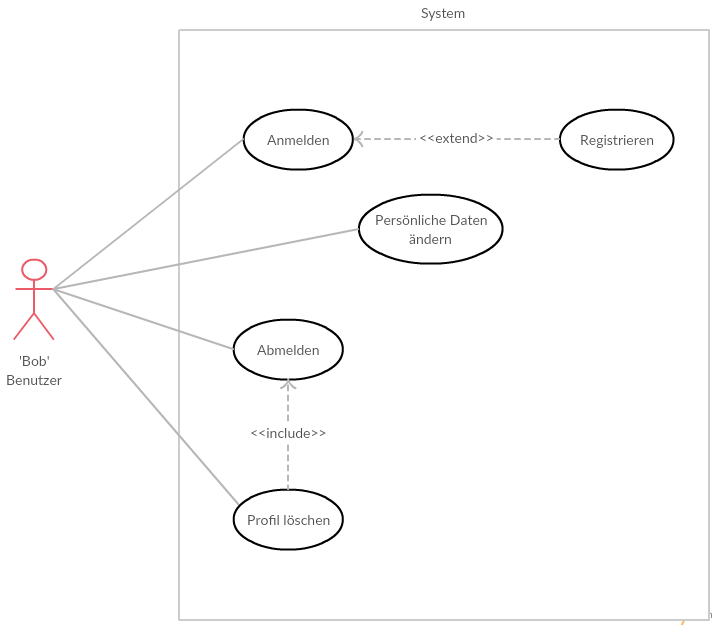
\includegraphics[width=.7\textwidth]{Use_Cases/use_case_Benutzerprofil.png}
	\caption{Use-Case Diagramm für Benutzerkontofunktionen}	
\end{figure}

\subsubsection{Funktionen}

\begin{enumerate}[label={\textbf{/F\protect\threedigits{\theenumi}0/}}, leftmargin=*]
	
	\item \textit{Registrieren}\label{Registrieren} \\ Ein beliebiger Benutzer, der zuvor die App auf seinem Android-Ger"at installiert hat und einen Google-Account besitzt, kann sich in der App registrieren und ein Benutzeraccount erstellen. Dazu muss der Benutzer sich auf dem Anmeldescreen (vgl. Abbildung \ref{login}) mit einem existierenden Google-Account anmelden (vgl. \ref{Anmelden}). Wird diese Funktion zum ersten Mal ausgeführt, wird vom System automatisch ein neuer Account für diesen Benutzer angelegt und der Benutzer in diesen Account eingeloggt. Bevor der Benutzer die App nutzen kann, muss er bestätigen, dass er mit einer eventuellen unanonymisierten Veröffentlichung seines Standortes einverstanden ist (vgl. \ref{Anonymisierung}). Wird dies nicht bestätigt, schlägt die Registrierung fehl.
	Bei erfolgreicher Registrierung kann sich der Benutzer ab sofort mit seinem Google-Account im System anmelden und Zugriff auf seinen Benutzeraccount erlangen.

	 	
	\item \textit{Anmelden} \label{Anmelden} \\ Ein Benutzer kann sich mithilfe seines Google-Accounts im System anmelden. Dazu sind folgende Eingaben des Benutzers erforderlich:
	\begin{itemize}
		\item E-Mail Adresse mit der der Benutzer bei Google registriert ist
		\item Passwort des Google-Accounts des Benutzers
	\end{itemize}
	Sind die Angaben korrekt wird der Benutzer vom System in sein GO-Benutzeraccount eingeloggt. Der Benutzer bleibt eingeloggt, bis er die Funktion \ref{Abmelden} ausführt, dies gilt auch für das zwischenzeitliche Schließen der App.
	
	%\item \textit{Benutzerkennung anfordern} \\ Ein Benutzer kann, sollte er sein Passwort vergessen haben, seine Benutzerkennung anfordern und eine neues Passwort setzen. Wird auf dem Anmeldescreen (vgl. *GUI-Ansicht*) die 'Passwort vergessen'-Option gewählt, schickt der Server dem Benutzer eine SMS mit einem Zugangscode. Dieser Zugangscode ist 10min lang gültig. Der Benutzer gibt den Zugangscode ein und kann anschließend eine neues Passwort setzen. Danach loggt das System den Benutzer ein und lädt die Hauptansicht der Applikation. Beim nächsten Anmelden kann sich der Benutzer mit dem neuen Passwort anmelden.
	
	\item \colorbox{shadecolor}{\textit{Persönliche Daten ändern}\label{Persönliche Daten ändern}} \\ Das System speichert persönliche Daten der Benutzer (siehe  \ref{persönliche Daten}). Der Benutzer kann diese Daten ändern. Dazu ruft der Benutzer sein Profil auf und betätigt die Schaltfläche 'Profil bearbeiten'. In der sich öffnenden Aktivität kann der Benutzer die gewünschten Änderungen vornehmen und mit dem Button 'Profil speichern' sichern. Die geänderten Daten werden dann vom System übernommen.\\
Daten, die mit dem Google-Account des Benutzers verknüpft sind (E-Mail Adresse und Passwort zum Anmelden) können nicht geändert werden.
	
	\item \textit{Abmelden}\label{Abmelden} \\ Ein Benutzer kann sich aus seinem Account abmelden, indem er in der Einstellungs-Ansicht die Option 'Abmelden' auswählt. Das System meldet daraufhin den Benutzer von seinem Benutzerkonto ab und lädt die Anmelde-Ansicht (vgl. Abbildung \ref{login}).
	
	\item \textit{Benutzerkonto l"oschen}\label{Benutzerkonto löschen}\\
	Ein Benutzer hat die Möglichkeit seinen Benutzeraccount zu löschen. Dazu ruft der Benutzer sein Profil auf und betätigt den Button 'Profil löschen'. Das System fragt den Benutzer ob das Konto wirklich gelöscht werden soll. Wird dies bestätigt so wird der Benutzer von dem System aus seinem Account ausgeloggt. Anschließend löscht das System alle Daten des Benutzerkontos (vgl. \ref{Profildaten}) und entfernt den Benutzer aus sämtlichen Gruppen und GO's denen er zuvor beigetreten war.
\end{enumerate}

\subsection{Gruppenfunktionen}

\subsubsection{Übersicht}
Die Gruppenfunktionen erlauben das Erstellen, Verwalten und Löschen von Gruppen im System. Das System unterscheidet zwischen den Rollen Gruppenmitglied und Gruppenadministrator. Dabei ist ein Gruppenadministrator gleichzeitig auch ein Gruppenmitglied.

\begin{figure}[H]
	\centering
	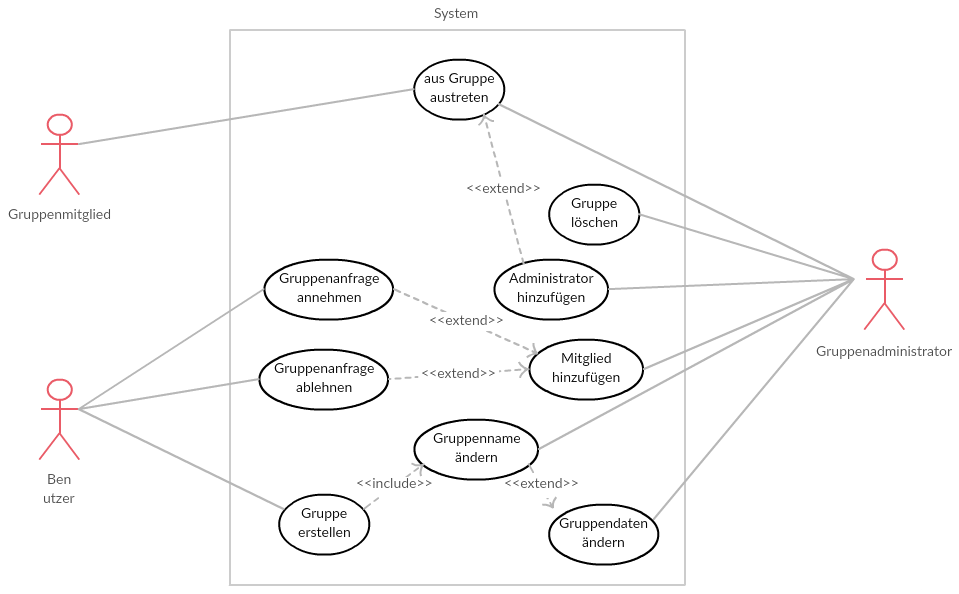
\includegraphics[width=1\textwidth]{Use_Cases/use_case_Gruppen.png}
	\caption{Use-Case Diagramm für Gruppenfunktionen}
\end{figure}



\subsubsection{öffentliche Funktionen}
Die im Folgenden beschriebenen Funktionen sind öffentlich, das bedeutet sie können von jedem Benutzer ausgeführt werden.
Im folgenden Abschnitt wird angenommen, dass der Benutzer ein Benutzerkonto besitzt und bereits im System eingeloggt ist.

\begin{enumerate}[label={\textbf{/F\protect\threedigits{\theenumi}0/}}, leftmargin=*, resume]
	\item \textit{Gruppen anzeigen}\label{Gruppen anzeigen} \\ %zählt hier "alle gruppen in denen man ist ansehen" als Funktion?
	Ein Benutzer kann sich alle Gruppen, in denen er zu diesem Zeitpunkt Mitglied ist, anzeigen lassen, indem er die Hauptansicht der App aufruft(vgl. Abbildung \ref{hauptansicht}).
	
	\item \textit{Gruppeninformationen abrufen}\label{Gruppeninfo anzeigen} \\%Mitglieder, Admin, aktuelle GOs
	Ein Benutzer, der Mitglied einer Gruppe ist, kann sich von der App Systeminformationen zu dieser Gruppe anzeigen lassen. Dazu wählt der Benutzer das Gruppenicon der gewünschten Gruppe in der Hauptansicht aus. Darauffolgend werden dem Benutzer vom System folgende Informationen über die Gruppe angezeigt:
	\begin{itemize}
		\item Gruppenname
		\item \colorbox{shadecolor}{Gruppenbild}
		\item \colorbox{shadecolor}{Gruppenbeschreibung}
		\item aktuelle Mitglieder der Gruppe (offene Gruppenmitgliedsanfragen werden nur den Administratoren der Gruppe angezeigt, ehemalige Mitglieder der Gruppe werden nicht angezeigt)
		\item aktuelle Administratoren der Gruppe
		\item aktuelle \glspl{GO} der Gruppe %kann geklickt werden, um in die Ansicht des jeweiligen GOs zu gelangen --> Querverweis einfügen
	\end{itemize}
	
	\item \textit{Gruppe erstellen}\label{Gruppe erstellen}\\
	Ein User kann eine neue Gruppe erstellen. Dazu muss in der Hauptansicht die Auswahl "Gruppe erstellen" gewählt werden und anschließend ein Gruppenname angegeben werden. Der Ersteller der Gruppe wird automatisch zum (zu diesem Zeitpunkt) einzigen Gruppenmitglied und Administrator derselben. Um anschließend Mitglieder zu der Gruppe hinzuzufügen, muss die Funktion \ref{Mitglieder hinzufügen} aufgerufen werden.
	
	
	\item \textit{Aus Gruppe austreten}\label{aus Gruppe austreten}\\
	Ein \gls{Benutzer}, der Mitglied einer Gruppe ist, kann aus derselben austreten. Sollte der Benutzer einziger Administrator der Gruppe sein, muss zuerst ein weiteres aktuelles Mitglied der Gruppe zum Administrator ernannt werden, bevor diese Funktion ausgeführt werden kann (siehe Funktion \ref{Admin hinzufügen}). \\
	Um aus einer Gruppe auszutreten wird vom Benutzer in der Hauptansicht die Gruppeninformationsansicht der ausgewählten Gruppe aufgerufen (vgl. Abbildung \ref{gruppeninfo}) und anschlie"send auf den Button 'Gruppe verlassen' geklickt. Das System entfernt den Benutzer aus der Gruppe und die Funktion ist erfolgreich abgeschlossen. Die Gruppe bleibt im System für alle anderen Benutzer weiterhin bestehen.\\
	In dem Fall, dass der austretende Benutzer das einzige Mitglied der Gruppe ist (und somit auch Administrator), entfällt das Ernennen eines neuen Administrators vor dem Austritt und die Gruppe wird nach dem Ausführen dieser Funktion automatisch vom System gelöscht.
	
	\item \textit{Gruppenanfrage beantworten}\label{Gruppenanfrage beantworten} \\
	Diese Funktion setzt voraus, dass ein Benutzer eine Anfrage auf Gruppenmitgliedschaft von einem anderen Benutzer bekommen hat (vgl. Funktion \ref{Mitglieder hinzufügen}). Dem Benutzer werden offene Gruppenanfragen durch ein farblich hinterlegtes Gruppenicon in der Hauptansicht angezeigt. Durch Klicken auf das Icon wird die Funktion "Gruppenanfrage beantworten" gestartet. Der Benutzer hat zwei Möglichkeiten auf die Anfrage zu reagieren:
	\begin{itemize}
		\item \textit{Bestätigen} bestätigt der Benutzer die Anfrage, so wird er vom System der Gruppe hinzugefügt. Sie erscheint ab sofort in seiner Gruppenübersicht und der Benutzer hat die Befugnis sämtliche öffentlichen Gruppenfunktionen für die Gruppe aufzurufen.
		\item \textit{Ablehnen} lehnt der Benutzer die Anfrage ab, wird diese Gruppenanfrage aus der Hauptansicht gelöscht und dem Benutzer wieder die Hauptansicht gezeigt.
	\end{itemize}
Nach Beantwortung der Anfrage wird diese vom System gelöscht.
\end{enumerate}

\subsubsection{Administratorfunktionen}
Im Folgenden wird angenommen, dass der Benutzer in seinem Benutzerkonto angemeldet und der Administrator einer Gruppe ist.\\
Um eine der folgenden Funktionen ausführen zu können muss der Administrator zunächst in die Gruppeninformationsansicht wechseln (vgl. Abbildung \ref{gruppeninfo} und \ref{Gruppeninfo anzeigen}). Unter der Voraussetzung, dass es sich bei dem Benutzer um einen Administrator dieser Gruppe handelt, wird ihm eine Schaltfläche 'Gruppe bearbeiten' angezeigt. Die Betätigung dieser Schaltfläche startet eine Aktivität, die es dem Benutzer erlaubt Änderungen an der aktuellen Konfiguration der Gruppe vorzunehmen. Es wird im Folgenden Abschnitt angenommen, dass der Benutzer diese Aktivität bereits gestartet hat.

\begin{enumerate}[label={\textbf{/F\protect\threedigits{\theenumi}0/}}, leftmargin=*, resume]

	\item \textit{Gruppendaten "andern}\label{Gruppendaten ändern}\\
	Ein Administrator kann folgende Daten einer Gruppe ändern:
	\begin{itemize}
	\item Gruppenname
	\item \colorbox{shadecolor}{Gruppenbeschreibung}
	\item \colorbox{shadecolor}{Gruppenbild}
	\end{itemize}
	Dazu gibt er die Änderungen in dem jeweiligen Feld der Änderungsansicht ein und betätigt anschließend den Button 'Änderungen speichern'.
	
	\item \textit{Gruppenmitglied hinzuf"ugen}\label{Mitglieder hinzufügen} \\
	Ein Administrator kann einer Gruppe neue Mitglieder hinzufügen. Dazu wählt er den Button 'Mitglied hinzufügen' aus. Anschließend kann anhand der E-Mailadresse, die beim Login benutzt wurde, nach dem gewünschten Benutzer gesucht werden. Das System zeigt dem Administrator Benutzer an, deren E-Mailadresse der Gesuchten entsprechen. Der Administrator wählt den gewünschten Benutzer aus, woraufhin das System diesem Nutzer eine Gruppenanfrage sendet (siehe \ref{Gruppenanfrage beantworten}). Solange die Gruppenanfrage offen ist, wird das potentielle Gruppenmitglied für die Administratoren der Gruppe angezeigt (Status der Mitgliedschaft ist farblich gekennzeichnet), für normale Gruppenmitglieder sind offene Gruppenanfragen nicht sichtbar.
	
	\item \textit{Gruppenmitglied entfernen}\label{Gruppenmitglied entfernen}\\
	Ein Administrator kann beliebige Mitglieder der Gruppe entfernen, indem er in der Änderungsansicht der Gruppe das rote Minuszeichen neben dem zu entfernenden Benutzer anklickt und anschließend die Durchführung der Aktion bestätigt. Der ausgewählte Benutzer wird vom System aus der Gruppe entfernt.
	
	\item \colorbox{shadecolor}{\textit{Admin hinzuf"ugen}}\label{Admin hinzufügen} \\
	Ein Administrator kann ein weiteres Mitglied der Gruppe zum Administrator ernennen. Dazu wählt er den 'Als Admin hinzufügen'-Option neben dem gewünschten Gruppenmitglied aus. Das System ändert die Rolle des Gruppenmitglieds zu 'Administrator'. Das Gruppenmitglied kann ab sofort alle Funktionen eines Administrators der Gruppe ausführen. Ein Administrator kann den Administrator-Status von anderen Administratoren nicht wieder entfernen.
	
	\item \textit{Gruppe l"oschen}\label{Gruppe löschen} \\
	Ein Administrator kann eine Gruppe löschen indem er den 'Gruppe löschen'-Button auswählt. Das System löscht die Gruppe. Sie wird ab diesem Zeitpunkt nicht mehr in der Gruppenansicht der Mitglieder angezeigt. Mitglieder erhalten keine Benachrichtigung über die Löschung der Gruppe.
	
\end{enumerate}
	
\subsection{GO-Funktionen}

\subsubsection{Übersicht}
Die GO-Funktionen erlauben das Erstellen, Verwalten und Löschen von sogenannten GOs, also Events bei denen die Standorte der \gls{GO-Teilnehmer} von System verfolgt und in der App angezeigt werden. Das System unterscheidet zwischen zwei Rollen: Gruppenmitglieder und GO-Verantwortliche. GO-Verantwortliche sind gleichzeitig auch Gruppenmitglieder, sind aber bei der Änderung ihres Teilnahmestatus in der Funktionalität eingeschränkt (nähere Erläuterung im folgenden Abschnitt).

	\begin{figure}[H]
		\centering
		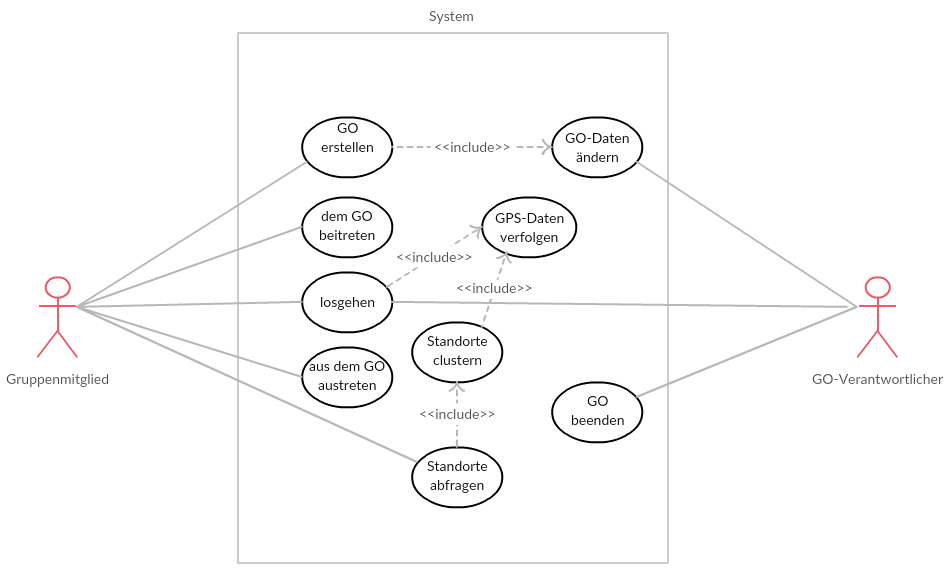
\includegraphics[width=1\textwidth]{Use_Cases/use_case_GO.png}
		\caption{Use-Case Diagramm für GO-Funktionen}
	\end{figure}

 

\subsubsection{öffentliche Funktionen}
Die in diesem Abschnitt beschriebenen Funktionen sind öffentlich, das bedeutet sie können von jedem Benutzer, der Mitglied einer Gruppe ist ausgeführt werden.
Im Folgenden wird angenommen, dass der Benutzer in seinem Benutzerkonto angemeldet und Mitglied einer Gruppe ist.

\begin{enumerate}[label={\textbf{/F\protect\threedigits{\theenumi}0/}}, leftmargin=*, resume]	

	\item \textit{GOs anzeigen}\label{GOs anzeigen} Ein Benutzer kann sich vom System seine GOs anzeigen lassen. Dies geschieht auf eine Art: \\
		Der Benutzer wählt die Detailansicht einer seiner Gruppe. Hier wird ihm eine Liste aller GOs dieser Gruppe angezeigt, unabhängig von seinem Teilnahmestatus für dieses GO.
	
	\item \textit{GO-Informationen abrufen}\label{GO-Informationen abrufen} \\
	Ein Benutzer dessen Teilnahmestatus 'Bestätigt' oder 'Unterwegs' ist, kann im System gespeicherte Informationen zu einem GO abrufen (vgl. \ref{GO-Daten}), indem er die Detailansicht des GOs, durch Klicken auf das GO-Icon in der GO-Hauptansicht oder der Gruppendetailansicht (vgl. Abbildung \ref{gruppendetailansicht}), anruft.

	\item \textit{GO erstellen}\label{GO erstellen} \\
	Jedes Mitglied einer Gruppe kann für diese Gruppe ein GO erstellen. Dazu wählt der Benutzer in der jeweiligen Gruppendetailansicht die Option 'GO erstellen' und übergibt dem System folgende Informationen:
	\begin{itemize}
		\item GO-Name
		\item \colorbox{shadecolor}{Beschreibung}
		\item Startzeitpunkt
		\item Endzeitpunkt 
		\item Zielpunkt (optional)
		\item \colorbox{shadecolor}{Clustering-Schwellwert (vgl. \ref{Clustering})}
	\end{itemize}
Der Startzeitpunkt darf nicht in der Vergangenheit liegen.\\
Hat der Benutzer die Angaben bestätigt, wird vom System ein neues GO erstellt und in den Mitgliedern der Gruppe in der Gruppendetailansicht angezeigt. Der Teilnahmestatus aller Gruppenmitglieder wird standardmäßig auf 'Abgelehnt' gesetzt. Der Teilnahmestatus des GO-Verantwortlichen wird auf 'Bestätigt' gesetzt.
Das GO wird den Mitgliedern der Gruppe in der Gruppendetailansicht angezeigt.
Der Ersteller des GOs ist während dem gesamten \gls{GO-Lifecycle} der GO-Verantwortliche. Es kann für ein GO keine weiteren GO-Verantwortlichen geben.
	%TODO abgelehnt nur von Bestätigt erreichbar, und nicht von unterwegs
	\item \textit{Teilnahmestatus ändern}\label{Teilnahmestatus} \\
	Das System weist für jedes GO jedem Gruppenmitglied einen Teilnahmestatus zu. Dieser lautet entweder
	\begin{itemize}
		\item Abgelehnt: Der Benutzer nimmt an dem GO nicht teil
		\item Bestätigt: Der Benutzer nimmt an dem GO teil
		\item Unterwegs: Der Benutzer nimmt an dem GO teil und ist bereits losgegangen
	\end{itemize}
Durch folgende Funktionen kann ein Benutzer seinen Teilnahmestatus in einem GO ändern.

	\begin{itemize}
	\item (a) \textit{Dem Event beitreten} \label{GO-Anfrage} \\
	Mitglieder einer Gruppe können zu jeder Zeit einem aktuellen GO der Gruppe beitreten. Dazu wird vorausgesetzt, dass der aktuelle Teilnahmestatus des Gruppenmitglieds 'Abgelehnt' ist. In der Gruppendetailansicht kann der Benutzer die Option 'Beitreten' des gewünschten GOs anklicken. Das System wird  veranlasst, den Teilnahmestatus des Benutzers auf 'Bestätigt' zu setzen. Sobald dies geschehen ist, kann der Benutzer die GO-Detailansicht (vgl. Abbildung \ref{goinfo}) aufrufen.
	
	\item (b) \textit{Losgehen}\label{losgehen} \\
	Um diese Funktion ausführen zu können, muss der Teilnahmestatus des Benutzers auf 'Bestätigt' gesetzt sein. Sobald der Button 'Losgehen' betätigt wurde wird der Teilnahmestatus des Benutzers vom System auf 'Unterwegs' gesetzt und die GPS-Verfolgung des Benutzers wird aktiviert und für andere GO-Mitglieder, deren Teilnahmestatus 'Bestätigt' oder 'Unterwegs' ist, sichtbar. Sobald der Startzeitpunkt eintritt, wird der Teilnahmestatus von Benutzern, die 'Bestätigt', aber noch nicht 'Unterwegs' sind, automatisch auf 'Unterwegs' gesetzt.
	
	\item (c) \textit{Aus Event austreten}\label{austreten} \\
Ein Benutzer, dessen Teilnahmestatus des GOs 'Bestätigt' oder 'Unterwegs' ist, kann seinen Status auf 'Abgelehnt' setzen, indem er in der GO-Detailansicht den Button 'Aus Event austreten' klickt. Das System setzt den Teilnahmestatus des Benutzers auf 'Abgelehnt'. Sollte die GPS-Verfolgung dieses GOs bereits aktiviert worden sein, wird sie vom System deaktiviert. Das System lädt die GO-Hauptansicht des Benutzers.
	
	\item (d) \textit{Anhalten}\label{anhalten} \\
	Ein Benutzer dessen Teilnahmestatus 'Unterwegs' lautet kann diesen zurück auf 'Bestätigt' setzen, indem er die Option 'Anhalten' auswählt. Das System ändert den Teilnahmestatus und stoppt die GPS-Verfolgung des Benutzers.
	
	\end{itemize}
	
	Bemerkung: Ein GO-Verantwortlicher kann nicht aus dem GO austreten. Der Teilnahmestatus eines GO-Verantwortlichen kann nur 'Bestätigt' oder 'Unterwegs' lauten.\\
	
	\begin{figure}[H]
		\centering
			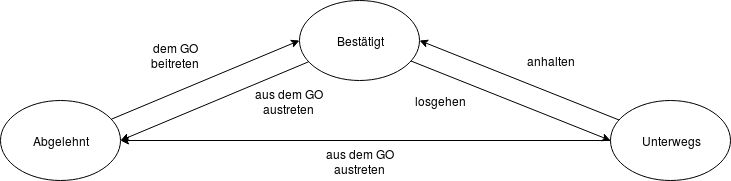
\includegraphics[scale=0.55]{res/Teilnahmestatus.png}
		\caption{Übergangsdiagramm für GO-Teilnehmerstatus}	
	\end{figure}
	
	
	\item \textit{Standorte abfragen}\label{Standorte abrufen} \\
	Ein Benutzer dessen Teilnahmestatus 'Bestätigt' oder 'Unterwegs' ist, kann, bei gestarteten GOs, die Standorte der Gruppenmitglieder abrufen, deren Teilnahmestatus 'Unterwegs' ist. Dazu ruft er die GO-Detailansicht auf (vgl. Abbildung \ref{godetailansicht}). Das System zeigt auf einer Karte die anonymisierten und ggf. zu Clustern zusammengefassten Standorte der losgegangen Benutzer an (vgl. \ref{Clustering}).
	
\end{enumerate}

\subsubsection{Funktionen für GO-Verantwortliche}
Im Folgenden wird angenommen, dass der Benutzer in seinem Benutzerkonto angemeldet ist und der Verantwortliche eines GOs ist.

\begin{enumerate}[label={\textbf{/F\protect\threedigits{\theenumi}0/}}, leftmargin=*, resume]	
	\item \textit{GO-Daten ändern}\label{GO Daten ändern} \\
	Der GO-Verantwortliche kann auch nach Erstellung des GOs die/den
	\begin{itemize}
		\item GO-Bezeichnung
		\item Startzeitpunkt
		\item Endzeitpunkt
		\item Zielpunkt
		\item \colorbox{shadecolor}{Clustering-Schwellwert (vgl. \ref{Clustering})}
	\end{itemize}
	ändern. Der neue Startzeitpunkt darf nicht in der Vergangenheit liegen. Sobald die Änderungen vom Benutzer bestätigt wurden, werden sie vom System übernommen und den Mitgliedern des GOs angezeigt, wenn diese die GO-Detailansicht aufrufen. Die GO-Daten können nicht mehr geändert werden, sobald der Startzeitpunkt eingetreten ist.
	
	\item \textit{GO beenden}\label{GO beenden} \\
	Ein GO kann vom GO-Verantwortlichen vorzeitig beendet werden durch Klicken des Buttons 'GO beenden' in der GO-Detailansicht. Es spielt für diese Funktion keine Rolle, ob der Startzeitpunkt bereits eingetreten ist oder nicht. Das System registriert das GO als beendet und stoppt die Standortverfolgung aller GO-Teilnehmer. Anschließend wird das GO vom System gelöscht. \\
	Wird das GO nicht vom GO-Veratnwortlichen vorzeitig beendet, wird es bei Erreichen des Endzeitpunkts automatisch vom System beendet. Das System führt dabei die gleichen Aktionen aus wie beim Beenden durch den GO-Verantwortlichen.
	
\end{enumerate}

\subsubsection{Systemfunktionen}
Die im folgenden beschriebenen Funktionen werden vom System ausgeführt, ohne das die Ausführung von einer direkten Interaktion mit dem Benutzer ausgelöst muss.
\begin{enumerate}[label={\textbf{/F\protect\threedigits{\theenumi}0/}}, leftmargin=*, resume]	
	
	\item \textit{Standorte verfolgen}\label{Standorte verfolgen}\\
	Das System verfolgt die Standorte aller Benutzer, dessen Teilnahmestatus für das GO auf 'Unterwegs' gesetzt ist. Die Standortverfolgung ist so lange aktiviert, bis sich der Teilnahmestatus des Benutzers ändert oder das GO beendet wird. Sie wird auch weiter durchgeführt, sollte der Benutzer die App nur im Hintergrund ausführen.
	
	\item \textit{\gls{Clustering}}\label{Clustering} \\
	Ist der Teilnahmestatus eines Benutzers in einem aktiven GO auf 'Unterwegs' gesetzt, beginnt das System den Standort dieses Benutzers zu erfassen. Die Standorte der losgegangenen Benutzer werden gegebenenfalls geclustert, sodass in der App nicht der Standort der einzelnen Benutzer, sondern die gemittelte Position dieser Benutzer angezeigt wird. Die Positionen mehrerer Benutzer werden zu einem Cluster zusammengefasst, sobald die Distanz der einzelnen Personen zum Zentrum des Clusters einen kritischen Schwellwert unterschreitet. \\ 
	
	\colorbox{shadecolor}{\parbox{.9\textwidth}{Dieser Schwellwert kann in den GO-Daten vom GO-Verantwortlichen bestimmt werden.}}\\
	
	 Es werden dem Benutzer beim Abrufen der Standorte (\ref{Standorte abrufen}) in einem GO die errechneten Standortcluster der anderen Benutzer angezeigt und wie viele Benutzer sich jeweils in einem Cluster befinden. Die Standorte von Benutzern, die sich nicht in der Nähe von anderen Benutzern befinden, werden nicht-geclustert dargestellt.
	
\item \textit{Anonymisierung der Benutzer}\label{Anonymisierung} \\ Die Funktionalität des Systems soll die Anonymität des Benutzers bestmöglich sicherstellen. Dazu sind folgende Funktionen der App zu implementieren:
		\begin{itemize}
			\item Die Standorte der Benutzer während eines GOs werden auf der Karte ohne den jeweiligen Benutzernamen angezeigt und bei ausreichender geographischer Nähe nur in Clustern dargestellt
			\item \colorbox{shadecolor}{\parbox{0.85\textwidth}{Die Genauigkeit der Standortbestimmung kann durch den Clustering-Schwellwert von dem GO-Verantwortlichen selbst bestimmt werden.}}
			\item \colorbox{shadecolor}{\parbox{.85\textwidth}{Bei GOs, bei denen weniger als 3 Benutzer die Standortverfolgung aktiviert haben, erhält der Benutzer beim Losgehen eine Warnung: er kann den Start der Standortverfolgung solange verzögern, bis mindestens 2 andere Benutzer ebenfalls losgegangen sind.}}
			\item Der automatische Start der Standortverfolgung bei Eintreten des Startzeitpunkts wird im Fall von weniger 3 losgegangen Benutzern nicht ausgeführt. Die Benutzer müssen manuell die Standortverfolgung durch Änderung des Teilnahmestatus auf 'Unterwegs' aktivieren.
			\item Benutzer haben zu jeder Zeit die Möglichkeit die Standortverfolgung zu beenden, indem sie ihren Teilnahmestatus auf 'Abgelehnt' oder 'Bestätigt' setzen.
		\end{itemize}
		Bemerkung: In Ausnahmefällen kann die Anonymität eines Benutzers nicht garantiert werden (etwa, wenn er sich als einziger nicht in der Nähe der anderen GO-Teilnehmer befindet oder das GO nur sehr wenige Teilnehmer hat). Das System weist den Benutzer bei erstmaliger Anmeldung auf diese Tatsache hin. Der Benutzer muss sich damit einverstanden erklären, bevor er die App nutzen kann (vgl. \ref{Registrieren}).
		
\end{enumerate}

\subsection{Sonstiges}
Im Folgenden wird angenommen, dass der Benutzer in seinem Benutzerkonto angemeldet ist.

\begin{enumerate}[label={\textbf{/F\protect\threedigits{\theenumi}0/}}, leftmargin=*, resume]	
 \item \colorbox{shadecolor}{\textit{Benachrichtigungen senden}}\label{Benachrichtigungen senden}\\
	Die App sendet dem Benutzer \glspl{Android-Benachrichtigung} bei folgenden Ereignissen:
	\begin{itemize}
		\item Der Benutzer wurde zu einer Gruppe hinzugefügt
		\item In einer Gruppe des Benutzers wurde ein GO erstellt
		\item ein GO des Benutzers ist gestartet
	\end{itemize}
	\item \colorbox{shadecolor}{\textit{Benachrichtigungseinstellungen ändern}}\label{Benachrichtigungseinstellungen ändern} \\
	Der Benutzer kann entscheiden, ob er Android-Benachrichtigungen von der App erhalten will oder nicht. Er kann dies selbst über einen Slider in der Einstellungs-Ansicht ändern. Die default-Einstellung ist 'stumm', d.h. der Benutzer erhält keine Benachrichtigungen der App auf seinem Android-Gerät.
	\item \textit{About-Seite anzeigen}\label{About} \\
	Der Benutzer kann eine 'About'-Seite aufrufen, die allgemeine Informationen zur App beinhaltet.
	\item \textit{Lizenzinformationen anzeigen}\label{Lizenz} \\
	Der Benutzer kann Informationen zur Lizenz der App einsehen.
\end{enumerate}

\newpage
\section{Produktdaten}

\begin{enumerate}[label={\textbf{/D\protect\threedigits{\theenumi}0/}}, leftmargin=*]
	\item \textit{Profildaten} \label{Profildaten} \\Für jeden im System registrierten Benutzer m"ussen folgende Informationen gespeichert werden:
		\begin{itemize}
			\item \textit{Benutzerkennung}
				\begin{itemize}
					\item Benutzer-ID (eindeutig, erzeugt von der verwendeten Firebase Authentication)
					\item E-Mailadresse des zum Anmelden verwendeten Google-Accounts
				\end{itemize}
			\item \textit{Persönliche Daten} \label{persönliche Daten} 
			\begin{itemize}
			\item \gls{Benutzername} (Default-Wert: Name aus dem Google-Account)
			\item \colorbox{shadecolor}{Profilbild}
			\item Gruppen
		\end{itemize}
		\end{itemize}
	
	\item \textit{Gruppendaten} \\Für jede erstellte Gruppe müssen folgende Informationen gespeichert werden:
	\begin{itemize}
		\item Gruppen-ID (eindeutig)
		\item Gruppenname
		\item \colorbox{shadecolor}{Gruppenbild}
		\item \colorbox{shadecolor}{Gruppenbeschreibung}
		\item Mitglieder
		\item Administratoren
		\item offene Gruppenanfragen %--> wie sollte man länger ausstehende Anfragen verwalten?
		\item aktuelle GOs
	\end{itemize}
	\item \textit{GO-Daten} \label{GO-Daten} \\
	Für jedes erstellte GO müssen folgende Informationen gespeichert werden:
	\begin{itemize}
		\item GO-ID (eindeutig)
		\item GO-Verantwortlicher
		\item GO-Name
		\item \colorbox{shadecolor}{Beschreibung}
		\item Startzeitpunkt
		\item Endzeitpunkt
		\item Zielort (optional)
		\item \colorbox{shadecolor}{Clustering-Schwellwert}
		\item Gruppe, der das GO angehört
		\item Gruppenmitglieder mit Teilnahmestatus 'Abgelehnt'
		\item Gruppenmitglieder mit Teilnahmestatus 'Bestätigt'
		\item Gruppenmitglieder mit Teilnahmestatus 'Losgegangen'
		\item Standorte der losgegangenen Benutzer
	\end{itemize}
\end{enumerate}

\newpage
\section{Nichtfunktionale Anforderungen}
\begin{enumerate}[label={\textbf{/NF\protect\threedigits{\theenumi}0/}}, leftmargin=*]
		\item \textit{Anonymisierung des Standortes} \\
		Um den Datenschutz, beziehungsweise die Privatsphäre der Benutzer zu garantieren, findet die Lokalisierung und Mittlung der Standorte(via GPS) der Mitglieder einer Gruppe, die sich einem Event angeschlossen haben, erst ab einer Teilnehmerzahl von 3 statt. 
		
		\item \textit{Eventlimit} \\
		Die Anzahl an gleichzeitig möglichen GOs ist auf 10 GOs pro Gruppe beschränkt um mögliche Überlastungen des Servers durch Schadsoftware oder böswillige Nutzer zu verhindern.
		
		\item \textit{Mitgliederanzahl} \\
		Die App ist auf kleine Gruppen und Ansammlungen ausgelegt. Daher wird die Zuverlässigkeit nur bis zu einer maximalen Mitgliederanzahl von 50 Benutzern pro Gruppe garantiert.
		
		\item \textit{Menüsortierung} \\
		Sowohl Gruppenübersicht als auch die Übersicht der Gruppenmitglieder ist alphabetisch (anhand des Benutzernamens) sortiert. 
		
		\item \textit{Serverlimit} \\
		Der Server erlaubt einen zuverlässigen Dienst nur bis zu einem Maximum von 300 möglichen Gruppen und 5000 Nutzern. Werden diese Werte überschritten, kann die problemlose Abarbeitung von Serveranfragen nicht mehr garantiert werden.
		
		\item \textit{Standortaktualisierungszeit} \\
		Die Aktualisierung der Standortmittlung findet alle 8 Sekunden statt.
		
		\item \textit{Automatisches Ausloggen} \\
		Der Nutzer wird nicht automatisch ausgeloggt sollte die App inaktiv oder geschlossen werden. Nur im Falle, dass der Nutzer sich auf einem anderen Gerät einloggt wird er auf dem vorigen ausgeloggt.
		
		\item \textit{Startzeit} \\
		Die Startzeit der App sollte nicht länger als 5 Sekunden betragen. \\
		Referenzgerät: Samsung Galaxy S7 mit Android 7.0
		
		\item \textit{Ausfallzeiten} \\
		Der Dienst der App ist für maximal 3 Tage pro Jahr nicht verfügbar.
		
\end{enumerate}

\newpage
\section{Benutzeroberfläche}

Im untenstehenden Flowchart wird die Struktur der grafischen Benutzeröberfläche der App dargestellt (bei fehler- und konfliktfreier Benutzung). Sollte es zu Fehleingaben durch den Benutzer kommen, wird eine Fehlermeldung gegeben. Die aktuelle GUI-Ansicht wird weiterhin angezeigt.

\begin{figure}[H]
	\vspace{1cm}
	\centering
	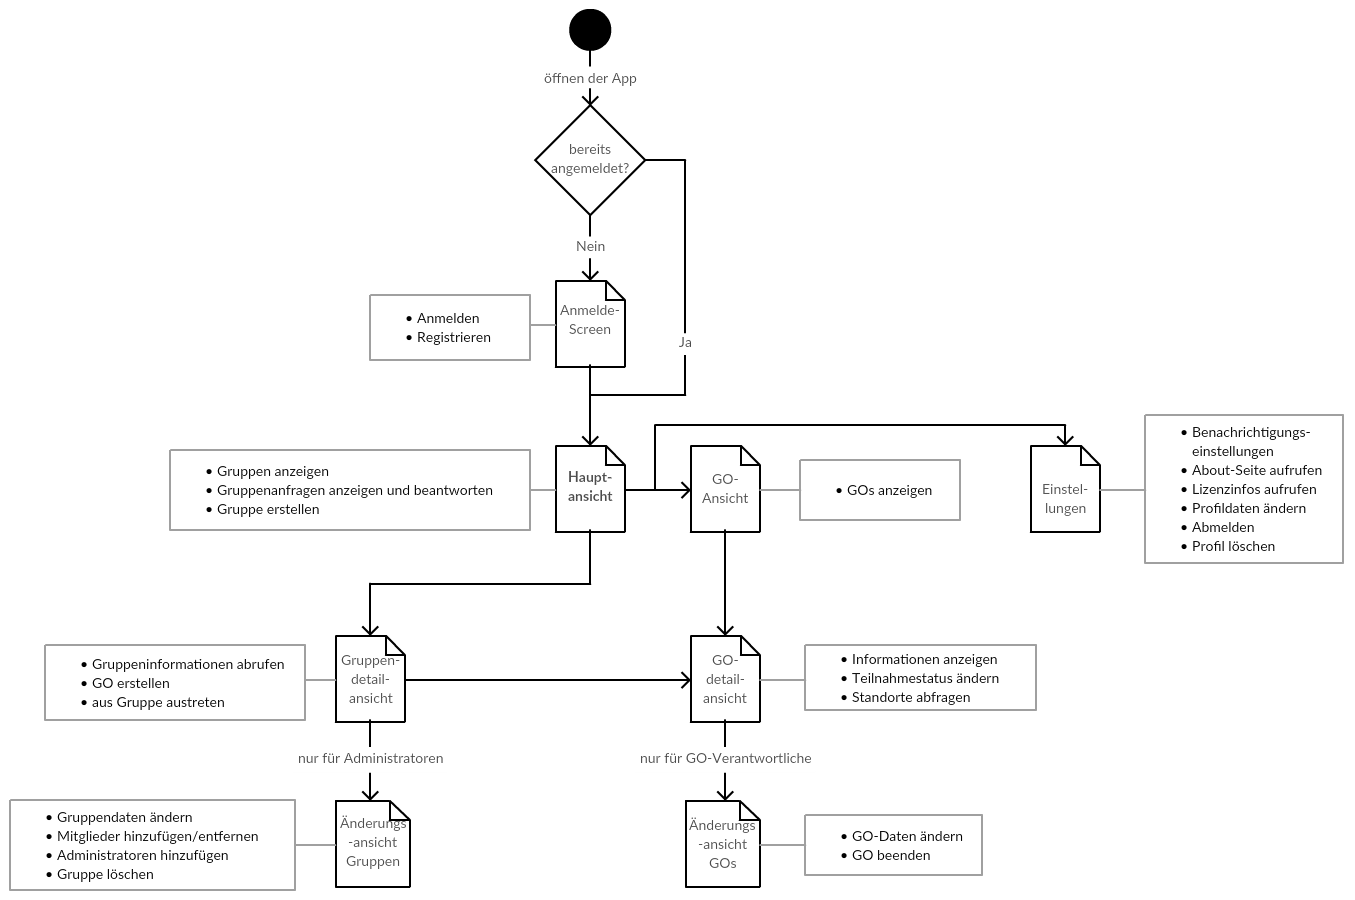
\includegraphics[width=\textwidth]{res/gui_flowchart.png}
	\caption{Flowchart der GUI-Ansichten der App}
	\vspace{1cm}
	\end{figure}

Die App besteht im Wesentlichen aus sechs Ansichten, die den Benutzer sämtliche Funktionen ausführen lassen (+ eine Login-Seite zum Anmelden/Registrieren). Diese werden durch verschiedene Änderungsansichten erweitert, sollte der Benutzer spezielle Rollen inne haben.

\newpage

Beim Starten der App, beziehungsweise nach erfolgreichem Anmelden/Registrieren auf der Login-Seite (vgl. Abbildung \ref{login}), gelangt der Benutzer auf die Hauptansicht der App (vgl. Abbildung \ref{hauptansicht}). Diese zeigt ihm alle Gruppen, in denen er aktuell Mitglied ist, plus aktuelle unbeantwortete Gruppenanfragen.

\begin{figure}[H]
  \vspace{1cm}
  \centering
  \begin{minipage}[b]{0.4\textwidth}
    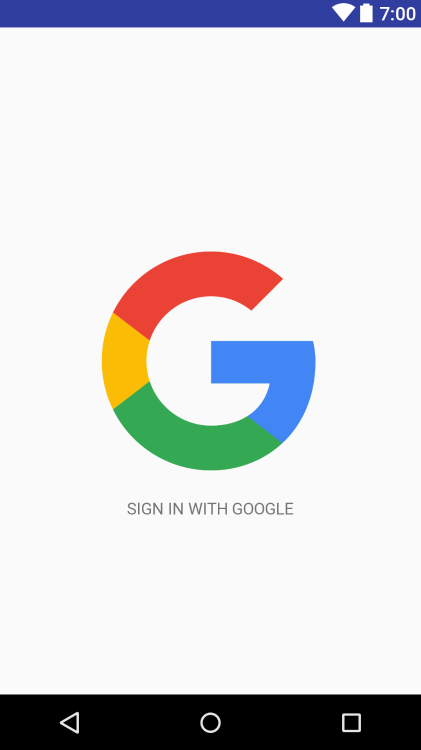
\includegraphics[width=\textwidth]{GUI/AndroidStudio/login_simple.PNG}
	\caption{Login-Seite}	\label{login} 
  \end{minipage}
  \hfill
  \begin{minipage}[b]{0.4\textwidth}
    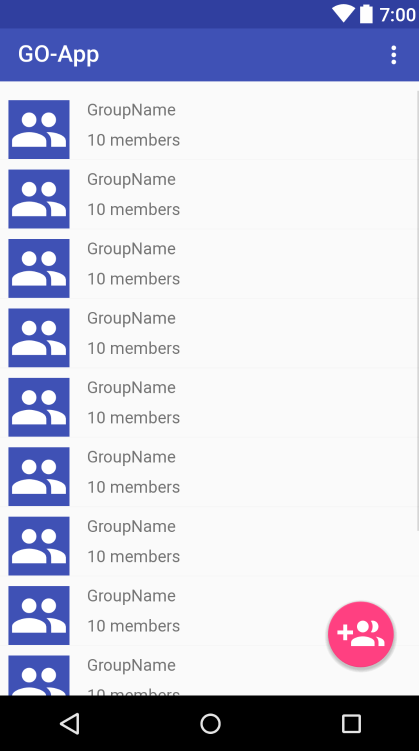
\includegraphics[width=\textwidth]{GUI/AndroidStudio/hauptansicht.PNG}
	\caption{Hauptansicht der App}	\label{hauptansicht}
  \end{minipage}
  \vspace{1cm}
\end{figure}

Von der Hauptansicht kann der Benutzer durch auswählen einer Gruppe in die Detailansicht dieser Gruppe gelangen (vgl. Abbildung \ref{gruppendetailansicht} und Abbildung \ref{gruppeninfo}). Sollte es sich bei dem Benutzer um einen Administrator handeln, so wird die Gruppendetailansicht erweitert durch die Änderungsansicht der Gruppe, in der spezielle Administratorfunktionen (z.B: Gruppendaten ändern, Mitglieder hinzufügen, etc.) ausgeführt werden können.

\begin{figure}[H]
  \vspace{1cm}
  \centering
  \begin{minipage}[b]{0.4\textwidth}
    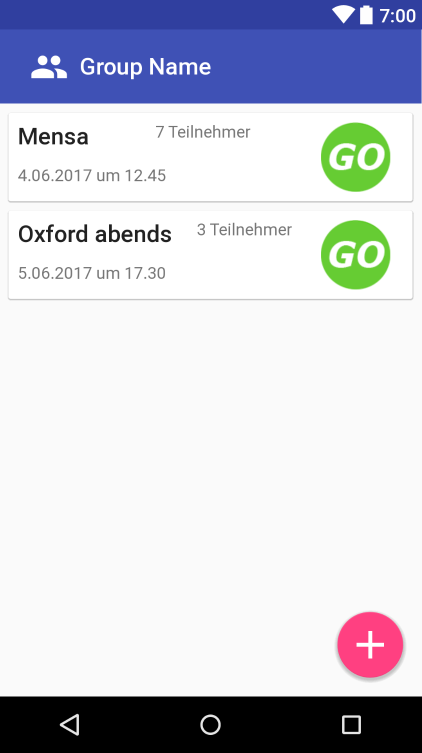
\includegraphics[width=\textwidth]{GUI/AndroidStudio/group_view.PNG}
	\caption{Gruppendetailansicht}\label{gruppendetailansicht}
  \end{minipage}
  \hfill
  \begin{minipage}[b]{0.4\textwidth}
    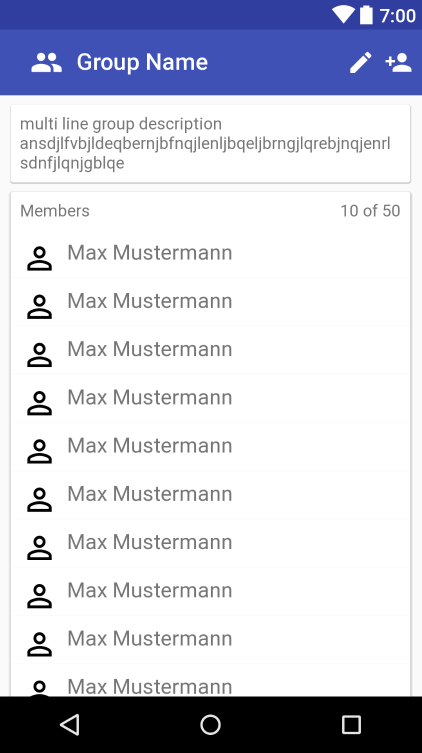
\includegraphics[width=\textwidth]{GUI/AndroidStudio/group_info.PNG}
	\caption{Gruppeninfo}\label{gruppeninfo}
  \end{minipage}
  \vspace{1cm}
\end{figure}

Ebenfalls von der Hauptseite ausgehend, kann der Benutzer auch zur GO-Ansicht wechseln. Es werden alle aktuellen GOs des Benutzers (mit Teilnahmestatus 'Bestätigt' oder 'Unterwegs') angezeigt. Durch Auswählen eines bestimmten GOs gelangt der Benutzer auf die Detailansicht dieses GOs (vgl. Abbildung \ref{godetailansicht}, und Abbildung \ref{goinfo}).\\
Eine zweite Möglichkeit die Detailansicht eines GOs aufzurufen ist, die Detailansicht der dazugehörigen Gruppe aufzurufen und in der GO-Auflistung (vgl. Abbildung \ref{gruppendetailansicht}) das entsprechende GO auszuwählen. \\

In der GO-Detailansicht, können alle zu einem GO gehörigen Funktionen ausgeführt werden. Handelt es sich bei dem Benutzer um den GO-Verantwortlichen, dann wird die GO-Detailansicht um die Änderungsansicht des GOs erweitert, in der spezielle Funktionen des GO-Veratnwortlichen (z.B. GO-Daten ändern, GO beenden) ausgeführt werden können.

\begin{figure}[H]
  \vspace{1cm}
  \centering
  \begin{minipage}[b]{0.4\textwidth}
    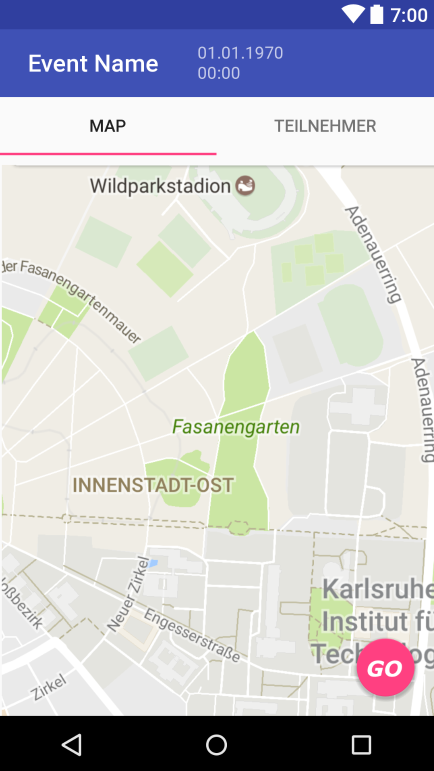
\includegraphics[width=\textwidth]{GUI/AndroidStudio/event_info_navi.PNG}
	\caption{Eventansicht, Karten-Tab}\label{godetailansicht}
  \end{minipage}
  \hfill
  \begin{minipage}[b]{0.4\textwidth}
    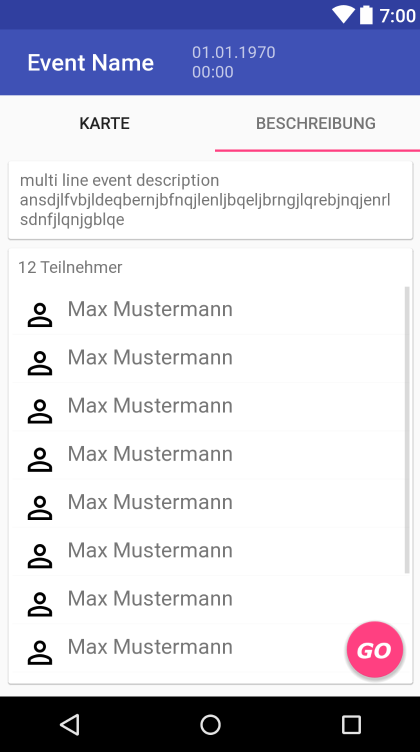
\includegraphics[width=\textwidth]{GUI/AndroidStudio/event_info_teilnehmer.PNG}
	\caption{Eventansicht, Eventinfo-Tab}\label{goinfo}
  \end{minipage}
  \vspace{1cm}
\end{figure}

Sonstige Funktionen, wie das Anzeigen der 'About'-Seite, oder Interaktionen mit dem eigenen Benutzerprofil (Ansehen, Ändern, Löschen, Abmelden) können vom Benutzer in der Einstellungsansicht ausgeführt werden, die ebenfalls von der Hauptseite aus erreichbar ist.

\newpage
\section{Qualitäts-Zielbestimmungen}
Bestimmung der Schwerpunkte in der Entwicklung dieser App:

\begin{table}[!h]
	\begin{center}
		\begin{tabular}{|c||c|c|c|}
			\hline  & Normaler Fokus & Hoher Fokus & Höchster Fokus\\
			\hline  Funktionalität & & & X \\
			\hline  Zuverlässigkeit & X & &\\
			\hline  Verständlichkeit & & X & \\
			\hline  Bedienbarkeit & & X &\\
			\hline  Effizienz & X & & \\
			\hline  Anpassbarkeit & & & X \\
			\hline  Kompatibilität & X & &\\
			\hline  Sicherheit & X & &\\
			\hline
		\end{tabular}
	\end{center}
\end{table}

\textbf{Hoher Fokus:}\\ Sowohl die Bedienbarkeit als auch die Verständlichkeit der App erhalten bei der Entwicklung einen großen Fokus, weil wir viel Wert auf ein simples und verständliches Design legen, um eine möglichst einfache und unkomplizierte Bedienung der App, sowie dass volle ausnutzen ihrer Funktionalitäten erlauben möchten.
	
\textbf{Höchster Fokus:}\\ Die Funktionalität ist ein Eckpunkt der größere Aufmerksamkeit bekommt, da der gesamte Wert der App sich anhand ihrer Operationsfähigkeit, ihrer Funktionen und der Umsetzung dieser messen lässt. Dabei spielt die Anpassbarkeit der App eine ebenso große Rolle, da das zukünftige Umsetzen neuer Ideen und möglicher Funktionen ein wichtiger Bestandteil der Wettbewerbsfähigkeit einer App ist.

% Funktionalität, Zuverlässigkeit, Benutzbarkeit, Effizienz, Änderbarkeit, Übertragbarkeit

\newpage
\section{globale Testfälle und Testszenarien}

\subsection{Erstellen, Verwalten, Löschen eines Benutzeraccounts}

\subsubsection*{Szenario 1}Bob will die GO-App nutzen. Dazu erstellt er einen Benutzeraccount, fügt persönliche Daten seinem Benutzerprofil hinzu und loggt sich anschließend wieder aus.\\

\textbf{Akteure:} Bob (Benutzer) \\

\textbf{Voraussetzungen: }Bob benutzt ein Smartphone, dass sämtliche Betriebsbedingungen erfüllt (vgl. \ref{Betriebsbedingungen}) erfüllt und auf dem die App installiert ist. Bob verfügt über ein gültiges Google-Konto.\\

\textbf{Testfälle:}
\begin{enumerate}[label={\textbf{/T\protect\threedigits{\theenumi}0/}}, leftmargin=*]
	\item\label{Registrieren-Test} \textbf{Aktion:} Bob öffnet die App, gibt die gültigen Anmeldedaten seines Google-Accounts ein und klickt auf den Button 'Sign In'. \\
									\textbf{Reaktion:} Das System lädt die Hauptansicht von Bobs Benutzerprofil.\\
									\textbf{getestete Funktion: }\ref{Registrieren}
	\item \textbf{Aktion:} Bob ist in seinem Benutzeraccount angemeldet. Bob öffnet seine Profilansicht und klickt auf den Button 'Profil ändern'. Er gibt in das Textfeld 'Benutzername' den Namen 'Bob' ein. Er klickt auf den Button 'Bild wählen'. Er wählt ein Bild aus dem Foto-Ordner des Android-Geräts aus. Er klickt auf den Button 'Änderungen speichern'. \\
		  \textbf{Reaktion:} Die neuen Daten werden in der Datenbank des Systems gespeichert. Sie werden in Bobs Profilansicht angezeigt.\\
		  \textbf{getestete Funktion: }\ref{Persönliche Daten ändern}
	\item \textbf{Aktion:} Bob ist in seinem Benutzeraccount angemeldet. Bob öffnet die Ansicht 'Einstellungen' und klickt auf das Feld 'Abmelden'.\\
		  \textbf{Reaktion:} Das System lädt die Anmelde-Seite.\\
		  \textbf{getestete Funktion: }\ref{Abmelden}
\end{enumerate}

\subsubsection*{Szenario 2}Bob will die App GO nicht mehr benutzen. Er will deshalb seinen Benutzeraccount löschen. \\

\textbf{Akteure:} Bob (Benutzer) \\

\textbf{Voraussetzungen: }Bob besitzt einen gültigen GO-Benutzeraccount.\\

\textbf{Testfälle:}
\begin{enumerate}[label={\textbf{/T\protect\threedigits{\theenumi}0/}}, leftmargin=*, resume]
	\item \textbf{Aktion:} Bob meldet sich in seinem Benutzeraccount an. \\
	\textbf{Reaktion:} Das System lädt die Hauptansicht von Bobs Profil.\\
	\textbf{getestete Funktion:} \ref{Anmelden}
	\item \textbf{Aktion:} Bob ist in seinem Benutzeraccount angemeldet. Er öffnet seine Profilansicht und klickt auf den Button 'Profil löschen'.\\
	\textbf{Reaktion:} Bobs Daten werden aus der Datenbank gelöscht. Die App lädt die Anmelde-Seite.\\
	\textbf{getestete Funktion:} \ref{Benutzerkonto löschen}
\end{enumerate}

\subsection{Erstellen, Verwalten, Löschen einer Gruppe}

\subsubsection*{Szenario 3} Bob, Alice und Peter wollen gemeinsam eine Gruppe erstellen, um ihre Treffen organisieren zu können. Bob soll der Administrator dieser Gruppe sein.\\

\textbf{Akteure:} Bob (Administrator), Alice (Gruppenmitglied), Peter (Gruppenmitglied) \\

\textbf{Voraussetzungen:} Bob, Alice und Peter verfügen über einen gültigen GO-Benutzeraccount.\\

\textbf{Testfälle:}
\begin{enumerate}[label={\textbf{/T\protect\threedigits{\theenumi}0/}}, leftmargin=*, resume]
	\item \textbf{Aktion:} Bob klickt in der Gruppenansicht auf das Feld 'neue Gruppe'. Er gibt in das Eingabefeld den Gruppennamen 'Foo' ein und bestätigt die Eingabe.\\
	\textbf{Reaktion:} Das System lädt die Gruppendetailansicht der Gruppe 'Foo'. Bob ist das einzige Mitglied und Administrator.\\
	\textbf{gestestete Funktion:} \ref{Gruppe erstellen}
	\item \textbf{Aktion:} Bob öffnet die Gruppendetailansicht und klickt auf den Button 'Gruppe bearbeiten'. Er gibt den Gruppennamen 'Bar' und die Gruppenbeschreibung 'FooBar' ein.\\
	\textbf{Reaktion:} Die neuen Gruppendaten werden in der Gruppendetailansicht angezeigt.\\
	\textbf{gestestete Funktion:} \ref{Gruppendaten ändern}
	\item \textbf{Aktion:} Bob öffnet die Gruppenansicht der App.\\
	\textbf{Reaktion:} Es wird die Gruppe 'Bar' angezeigt.\\
	\textbf{getestete Funktion: }\ref{Gruppen anzeigen}
	\item \textbf{Aktion:} Bob öffnet die Gruppendetailansicht und klickt auf das Feld 'Mitglied hinzufügen'. Er gibt in das Suchfeld Alice's E-Mailadresse ein. Er wählt aus den Suchresultaten Alice's Profil aus. Er wiederholt den Vorgang, um Peter zur Gruppe hinzuzufügen.\\
	\textbf{Reaktion:} In der Gruppendetailansicht von Bob werden Alice und Peter als potenzielle Mitglieder angezeigt. Alice und Peter erhalten Gruppenanfragen.\\
	\textbf{getestete Funktion: }\ref{Mitglieder hinzufügen}
	\item \textbf{Aktion:} Alice hat eine Gruppenanfrage für die Gruppe 'Bar' bekommen. Sie bestätigt die Gruppenanfrage.\\
	\textbf{Reaktion:} Die Gruppenanfrage wird aus Alice's Gruppenansicht gelöscht. Die App öffnet die Gruppendetailansicht. In Bobs Gruppendetailansicht wird Alice als Gruppenmitglied angezeigt.\\
	\textbf{getestete Funktion:} \ref{Gruppenanfrage beantworten}
	\item \textbf{Aktion:} Peter hat eine Gruppenanfrage für die Gruppe 'Bar' bekommen. Er lehnt die Gruppenanfrage ab.\\
	\textbf{Reaktion:} Die Gruppenanfrage wird aus Peters Gruppenansicht entfernt. In Bobs Gruppendetailansicht wird Peter nicht mehr als potenzielles Mitglied angezeigt.\\
	\textbf{getestete Funktion: }\ref{Gruppenanfrage beantworten}
	\item \textbf{Aktion:} Alice ruft die Gruppendetailansicht auf.\\
	\textbf{Reaktion:} Ihr werden folgende Informationen angezeigt:
	\begin{itemize}
		\item Gruppenname: Bar
		\item Gruppenbeschreibung: FooBar
		\item Mitglieder: Bob, Alice
		\item Administratoren: Bob
		\item aktuelle GOs: leer
	\end{itemize}
	\textbf{getestete Funktion: }\ref{Gruppeninfo anzeigen}
\end{enumerate}

\subsubsection*{Szenario 4}Nach dem Event wollen Bob, Alice und Peter die Gruppe 'Bar' wieder auflösen.\\

\textbf{Voraussetzungen: }Bob, Alice und Peter verfügen über je einen gültigen GO-Benutzeraccount. Bob, Alice und Peter sind gemeinsam Mitglieder der Gruppe 'Bar'. Bob ist Administrator, Alice und Peter sind Gruppenmitglieder.\\

\textbf{Akteure:} Bob (Administrator), Alice (Gruppenmitglied), Peter (Gruppenmitglied) \\

\textbf{Testfälle:}
\begin{enumerate}[label={\textbf{/T\protect\threedigits{\theenumi}0/}}, leftmargin=*, resume]
	\item \textbf{Aktion:} Bob wählt in der Gruppendetailansicht der Gruppe 'Bar' die Option 'Austreten'. \\
	\textbf{Reaktion:} Die Aktion schlägt fehl, da Bob der einzige Administrator der Gruppe ist.\\
	\textbf{getestete Funktion:} \ref{aus Gruppe austreten}
	\item \textbf{Aktion:} Bob wählt in der Gruppendetailansicht der Gruppe 'Bar' die Option 'Administrator hinzufügen'. Er wählt Alice als neuen Administrator aus.\\
	\textbf{Reaktion:} Alice wird in der Gruppendetailansicht als Administrator angezeigt. Alice wird in der Gruppendetailansicht die Möglichkeit zur Änderungsansicht zu wechseln, angezeigt.\\
	\textbf{getestete Funktion:} \ref{Admin hinzufügen}
	\item \textbf{Aktion:} Bob wählt in der Gruppendetailansicht der Gruppe 'Bar' die Option 'Austreten'.\\
	\textbf{Reaktion:} Die App lädt die Hauptansicht. Die Gruppe 'Bar' wird nicht mehr angezeigt. In Alice's Gruppedetailansicht wird Bob nicht mehr als Mitglied angezeigt.\\
	\textbf{getestete Funktion:} \ref{aus Gruppe austreten}
	\item \textbf{Aktion:} Alice entfernt Peter aus der Gruppe 'Bar'.\\
	\textbf{Reaktion:} Peter wird nicht mehr als Mitglied in der Gruppendetailansicht angezeigt. In Peters Hauptansicht wird die Gruppe 'Bar' nicht mehr angezeigt.\\
	\textbf{getestete Funktion:} \ref{Gruppenmitglied entfernen}
	\item \textbf{Aktion:} Alice wählt in der Gruppendetailansicht die Option 'Gruppe löschen'.\\
	\textbf{Reaktion:} Die App lädt die Hauptansicht. Bei sämtlichen Mitgliedern wird die Gruppe 'Bar' nicht mehr in der Hauptansicht angezeigt.\\
	\textbf{getestete Funktion:} \ref{Gruppe löschen}
\end{enumerate}

\subsection{Erstellen, Verwalten und Löschen eines GOs}

\subsubsection*{Szenario 5}Bob erstellt ein neues GO in der Gruppe 'Bar'. Alice tritt dem GO bei und bestätigt 10min vor dem Startzeitpunkt, dass sie losgegangen ist.\\

\textbf{Akteure:} Bob (GO-Verantwortlicher), Alice (Gruppenmitglied)\\

\textbf{Voraussetzungen: }Bob und Alice sind Mitglieder der Gruppe 'Bar'. Die Gruppe hat eine Gesamtmitgliederzahl von 5 Benutzern.\\

\textbf{Testfälle:}
\begin{enumerate}[label={\textbf{/T\protect\threedigits{\theenumi}0/}}, leftmargin=*, resume]
	\item\label{Go Test} \textbf{Aktion:} Bob erstellt ein GO mit folgenden Daten:
	\begin{itemize}
		\item Name: Mittagessen
		\item Beshcreibung: Mittagessen im Oxford Pub
		\item Startzeitpunkt: 15.09.17 12:00
		\item Endzeitpunkt: 15.09.2017 14:00
		\item Zielort: leer
		\item Clustering-Schwellwert: 100m
	\end{itemize}
	\textbf{Reaktion:} Die App lädt die Detailansicht des GOs. In der Gruppendetailansicht der Gruppe 'Bar' wird den Gruppenmitgliedern das GO angezeigt. Das GO wird in Bobs GO-Ansicht angezeigt.\\
	\item \textbf{Aktion:} Alice ruft die GO-Detailansicht auf, um sich über das GO zu informieren.\\
	\textbf{Reaktion:} Ihr werden die Informationen aus Testfall \ref{Go Test} angezeigt.\\
	\textbf{getestete Funktion:} \ref{GO erstellen}
	\item \textbf{Aktion:} Alice setzt ihren Teilnahmestatus auf 'Bestätigt'.\\
	\textbf{Reaktion:} Die App lädt die GO-Detailansicht. Alice wird den anderen GO-Teilnehmern in der Detailansicht als GO-Teilnehmerin angezeigt.\\
	\textbf{getestete Funktion:} \ref{Teilnahmestatus} (a)
	\item \textbf{Aktion:} Alice ruft die GO-Ansicht auf.\\
	\textbf{Reaktion:} Ihr wird das GO 'Mittagessen' aus der Gruppe 'Bar' angezeigt.\\
	\textbf{getestete Funktion:} \ref{GO-Informationen abrufen}
	\item \textbf{Aktion:} Alice setzt ihren Teilnahmestatus manuell auf 'Unterwegs'.\\
	\textbf{Reaktion:} Alice's Standort wird erfasst und in der Kartenansicht des GOs angezeigt.\\
	\textbf{getestete Funktion:} \ref{Teilnahmestatus} (b)
	\item \textbf{Aktion:} alle Gruppenmitgleider außer Bob sind bereits losgegangen. Der Startzeitpunkt tritt ein.\\
	\textbf{Reaktion:} Das System setzt Bobs Teilnahmestatus automatisch auf 'Unterwegs'. Bobs Standort wird erfasst und in der Kartenansicht des GOs angezeigt.\\
	\textbf{getestete Funktion: }\ref{Teilnahmestatus} (b)
	\item \textbf{Aktion:} alle Gruppenmitglieder außer Bob sind als Gruppe (geographisch nah beieinander) unterwegs.\\
	\textbf{Reaktion: }Bob kann die Standorte der anderen Gruppenmitglieder nur als Cluster auf der Karte sehen.\\
	\textbf{getestete Funktion:} \ref{Clustering}, \ref{Anonymisierung}, \ref{Standorte abrufen}, \ref{Standorte verfolgen}
	\item (a) \textbf{Aktion:} das GO wird von Bob manuell beendet. \\
	\textbf{Reaktion: }Die App lädt die Hauptansicht. Das Go wird in der Gruppendetailansicht, sowie der GO-Ansicht nicht mehr angezeigt. Es wird von keinem Teilnehmer mehr der Standort erfasst.\\
	\textbf{getestete Funktion:} \ref{GO beenden}\\
	 (b) \textbf{Aktion:} das GO endet zum Endzeitpunkt automatisch.\\
	 \textbf{Reaktion: }Die App lädt die Hauptansicht. Das Go wird in der Gruppendetailansicht, sowie der GO-Ansicht nicht mehr angezeigt. Es wird von keinem Teilnehmer mehr der Standort erfasst.\\	
	 \textbf{getestete Funktion:} \ref{GO beenden}
\end{enumerate}

\subsubsection*{Szenario 6} Die Pläne der Gruppe ändern sich. Bob muss die Details des GOs ändern. Letztendlich muss das Treffen komplett abgesagt werden, also wird das GO von Bob gelöscht.\\

\textbf{Akteure:} Bob (GO-Verantwortlicher)\\

\textbf{Voraussetzungen: }Bob hat zuvor ein GO erstellt mit den GO-Daten aus Testfall \ref{Go Test} und ist der GO-Verantwortliche. Das GO hat noch nicht begonnen.\\

\textbf{Testfälle:}
\begin{enumerate}[label={\textbf{/T\protect\threedigits{\theenumi}0/}}, leftmargin=*, resume]
	\item \textbf{Aktion:} Bob ruft die GO-Detailansicht auf und ändert den Startzeitpunkt des GOs von 15.09.17 12:00 auf 15.09.17 13:00\\
	\textbf{Reaktion:} Es wird die Detailansicht des GOs geladen. Der neue Startzeitpunkt wird angezeigt.\\
	\textbf{getestete Funktion:} \ref{GO Daten ändern}
	\item \textbf{Aktion:} Bob beendet das GO\\
	\textbf{Reaktion:} Die App lädt die Hauptansicht. Das GO wird nicht mehr in der Gruppendetailansicht angezeigt. Auch in der GO-Ansicht der GO-Teilnehmer wird es nicht mehr angezeigt.\\
	\textbf{getestete Funktion:} \ref{GO beenden}
\end{enumerate}

\subsubsection*{Szenario 7}Alice entfernt sich während des GOs von der Gruppe. Sie will nicht, dass man ihren Standort verfolgen kann, deshalb setzt sie ihren Teilnahmestatus von 'Unterwegs' auf 'Bestätigt'. Nach einer Weile entschließt sie sich nicht mehr zu der Gruppe zurückzukehren und verlässt das GO.\\

\textbf{Akteure:} Bob (GO-Verantwortlicher), Alice (Gruppenmitglied)\\

\textbf{Voraussetzungen: }Alice ist Mitglied einer Gruppe. Es findet aktuell ein GO statt. Alice's Teilnahmestatus für dieses GO lautet 'Unterwegs'.\\

\textbf{Testfälle:}
\begin{enumerate}[label={\textbf{/T\protect\threedigits{\theenumi}0/}}, leftmargin=*, resume]
	\item \textbf{Aktion:} Alice ändert ihren Teilnahmestatus auf 'Bestätigt'.\\
	\textbf{Reaktion:} Die App lädt die GO-Detailansicht. Alice's Standort wird nicht mehr erfasst. Ihr Standort ist für die anderen GO-Teilnehmer nicht mehr sichtbar.\\
	\textbf{getestete Funktion:} \ref{Teilnahmestatus} (d)
	\item \textbf{Aktion:} Alice ändert ihren Teilnahmestatus auf 'Abgelehnt'.\\
	\textbf{Reaktion:} Die App lädt die Hauptansicht. Alice wird den anderen GO-Teilnehmern nicht mehr als Teilnehmerin angezeigt.\\
	\textbf{getestete Funktion:} \ref{Teilnahmestatus} (c)
\end{enumerate}

\subsection{Sonstiges}

\subsubsection*{Szenario 8} Bob will sich über die App GO informieren und schaut sich dazu die About- und Lizenzinformnationsseiten der App an.\\

\textbf{Akteure:} Bob (Benutzer)\\

\textbf{Voraussetzungen:} Bob besitzt einen gültigen GO-Benutzeraccount.\\

\textbf{Testfälle:}
\begin{enumerate}[label={\textbf{/T\protect\threedigits{\theenumi}0/}}, leftmargin=*, resume]
	\item \textbf{Aktion:} Bob ruft die About-Seite der App auf.\\
	\textbf{Reaktion:} Die 'About'-Seite wird angezeigt.\\
	\textbf{getestete Funktion:} \ref{About}
	\item \textbf{Aktion:} Bob ruft die Lizenzinformationen der App auf.\\
	\textbf{Reaktion: }Die Lizenzinformationen werden angezeigt.\\
	\textbf{getestete Funktion:} \ref{Lizenz}
\end{enumerate}

\subsubsection*{Szenario 9} Bob und Alice erstellen gemeinsam eine neue Gruppe mit Alice als Administrator. Bob aktiviert die Benachrichtigungen der App, um zeitnah mitzubekommen, wenn es Neuigkeiten in der Gruppe gibt.\\

\textbf{Akteure: }Bob (Gruppenmitglied), Alice (Administrator)\\

\textbf{Voraussetzungen: }Bob und Alice besitzen beide einen gültigen GO-Benutzeraccount. Alice ist Administrator der Gruppe 'Foo'.\\

\textbf{Testfälle:}
\begin{enumerate}[label={\textbf{/T\protect\threedigits{\theenumi}0/}}, leftmargin=*, resume]
	\item \textbf{Aktion:} Bob ändert die Benachrichtigungseinstellungen in seinem Profil auf 'aktiv'.\\
	\textbf{Reaktion: }Die Einstellung wird vom System gespeichert. Der Vorgang ist für den Benutzer nicht sichtbar.\\
	\textbf{getestete Funktion:} \ref{Benachrichtigungseinstellungen ändern}
	\item \textbf{Aktion:} Alice fügt Bob der Gruppe 'Foo' hinzu.\\
	\textbf{Reaktion: }Bob bekommt eine Benachrichtigung auf seinem Android-Gerät.\\
	\textbf{getestete Funktion:} \ref{Benachrichtigungen senden}
	\item \textbf{Aktion:} Alice erstellt ein neues GO in der Gruppe 'Foo'.\\
	\textbf{Reaktion: }Bob bekommt eine Benachrichtigung auf seinem Android-Gerät.\\
	\textbf{getestete Funktion:} \ref{Benachrichtigungen senden}
	\item \textbf{Aktion:} Der Startzeitpunkt des GOs ist eingetreten.\\
	\textbf{Reaktion: }Bob bekommt eine Benachrichtigung auf seinem Android-Gerät.\\
	\textbf{getestete Funktion:} \ref{Benachrichtigungen senden}
\end{enumerate}
Mit diesen Testfällen sollen speziell die Benachrichtigungsfunktionen der App getestet und nicht die Funktionen zum Erstellen einer Gruppe/eines GOs. Für diese Testfälle ist sicherzustellen, dass diese Funktionen fehlerfrei funktionieren.

% \newpage
% \section{Anhang}

\newpage
\printglossary	
\end{document}



\grid
